\documentclass[10pt,a4paper]{article}
\usepackage[T1]{fontenc}
\usepackage[utf8]{inputenc}
\IfFileExists{lmodern.sty}{\usepackage{lmodern}}{\usepackage{mathptmx}}
\usepackage[margin=2.2cm]{geometry}
\usepackage{graphicx,booktabs,amsmath,amssymb,xcolor,listings,tikz,hyperref,caption}
\usepackage[expansion=false]{microtype}
\usetikzlibrary{positioning,arrows.meta,fit}
\hypersetup{colorlinks=true,linkcolor=blue!50!black,citecolor=blue!50!black,urlcolor=blue!50!black}
\lstdefinestyle{yaml}{basicstyle=\ttfamily\scriptsize,columns=fullflexible,frame=single,framerule=0.3pt,
  keywordstyle=\color{blue!60!black},commentstyle=\color{gray},showstringspaces=false,breaklines=true}
\newcommand{\CarbonAHystPct}{-0.5}
\newcommand{\CarbonAReactivePct}{8.8}
\newcommand{\CarbonBHystPct}{-2.6}
\newcommand{\CarbonBReactivePct}{3.9}
\newcommand{\CarbonSavingChurn}{91}
\newcommand{\CarbonSavingRetail}{92}
\newcommand{\CostAHystPct}{-0.6}
\newcommand{\CostAReactivePct}{69}
\newcommand{\CostBHystPct}{-1.0}
\newcommand{\CostBReactivePct}{58}
\newcommand{\CostExtraChurn}{5.6}
\newcommand{\CostExtraRetail}{11.1}
\newcommand{\CovData}{5/8}
\newcommand{\CovModel}{5/9}
\newcommand{\CovNonPlan}{21/31}
\newcommand{\CovOps}{9/9}
\newcommand{\CovPlan}{0/7}
\newcommand{\CovSoft}{2/5}
\newcommand{\CovTotal}{21/38}
\newcommand{\FeatEffective}{34}
\newcommand{\FeatLeaves}{50}
\newcommand{\FeatNoEffect}{Airflow, ArgoWorkflows, DataVersioning, ExperimentTracking, Industry40IoT, Kubeflow, Kubernetes, Retail, Serverless, TabularClassification}
\newcommand{\FeatTested}{44}
\newcommand{\JAHyst}{1.000}
\newcommand{\JAOracle}{0.983}
\newcommand{\JAReactive}{1.301}
\newcommand{\JBHyst}{1.009}
\newcommand{\JBOracle}{0.993}
\newcommand{\JBReactive}{1.271}
\newcommand{\JobCarbonAPct}{11}
\newcommand{\JobCarbonBPct}{2}
\newcommand{\MigAHyst}{0.4}
\newcommand{\MigAOracle}{3.1}
\newcommand{\MigAReactive}{102}
\newcommand{\MigBHyst}{0.5}
\newcommand{\MigBOracle}{1.9}
\newcommand{\MigBReactive}{90}
\newcommand{\NConstraints}{10}
\newcommand{\NFeatures}{69}
\newcommand{\NLeaves}{50}
\newcommand{\NLocations}{9}
\newcommand{\NOffers}{27}
\newcommand{\NProfiles}{4}
\newcommand{\NRules}{8}
\newcommand{\RatioMax}{80.6}
\newcommand{\RatioMin}{18.3}
\newcommand{\ScalMaxSeconds}{0.00}
\newcommand{\ScalMaxSteps}{30}

\newcommand{\tool}{\textsf{amlops}}

\title{From Variability Knowledge to Sovereign Multi-Cloud Deployment:\\
A Low-Code DSL for Adaptive MLOps Pipelines\\[4pt]
\large An industrial-partner contribution to the ANR AdaptiveMLOps project}
\author{Xavier Quesnot\\ GetCaaS, France\\ \texttt{xavier@getcaas.io}}
\date{Draft v0.1 --- \today\ --- for consortium review}

\begin{document}
\maketitle

\begin{abstract}
MLOps pipelines must be continuously retrained to cope with data and concept
drift, and increasingly operated across several cloud providers under cost,
carbon and sovereignty constraints. Designing them requires knowledge spread
across data scientists, ML engineers and operations engineers. Building on the
variability mapping and the SkeltyMLOps reference architecture produced within the
ANR AdaptiveMLOps project, we present \tool, an open-source prototype that
(i)~formalises MLOps variability as a feature model whose six top-level
categories come from a prior mapping study, complemented by documented
best-practice rules; (ii)~offers a two-level YAML domain-specific language in
which a non-expert writes a profile and objectives while an expert refines
features, steps and parameters; (iii)~derives a platform-independent pipeline
model following a software-process-line view, including executable coordination
contracts; (iv)~places pipeline steps across providers with an exact
multi-objective optimiser and compiles the result to Terraform, Argo Workflows
and CI artefacts; and (v)~re-places services and schedules drift-triggered
retraining at run time. We evaluate the prototype on four illustrative case
studies with an illustrative provider catalogue and synthetic environment traces.
Generated artefacts realise \CovNonPlan{} of the non-planning SkeltyMLOps
activities; \FeatEffective{} of \FeatTested{} testable leaf features have an
observable effect on the output, the others pinpointing missing generators.
Static carbon-aware placement cuts operational carbon by
\CarbonSavingChurn--\CarbonSavingRetail\% versus a cost-only placement for
\CostExtraChurn--\CostExtraRetail\% extra cost. In contrast, hourly re-placement of
serving components brings little: even a clairvoyant oracle improves the
normalised objective by at most \(\approx\)2\% over a static placement, while a
naive reactive policy migrates \(\approx\)\MigAReactive{} times a month and worsens it
by 27--30\%. We discuss what these results mean for the design of adaptive
MLOps tooling and what real industrial traces must now confirm.
\end{abstract}

\section{Introduction}
MLOps extends DevOps to the development and operation of ML-powered
software~\cite{kreuzberger2023,sculley2015}. Once deployed, models face changing
data distributions and degrade silently~\cite{gama2014}; pipelines therefore embed
monitoring, retraining triggers and redeployment. In practice these pipelines are
assembled from heterogeneous tools and platforms, and must satisfy
non-functional and organisational requirements: cost, latency, environmental
footprint, and, in Europe, data residency and qualified hosting (e.g.\ SecNumCloud
or HDS in France).

The ANR AdaptiveMLOps project (ANR-24-IAS2-0004) studies how domain engineering
(feature models, software product and process lines) and model-driven engineering
(MDE) can capture this variability and assist the design of new pipelines. Two
first results of the consortium frame this paper: a variability mapping study that
identified six variability categories and eight modelling requirements
R1--R8~\cite{elhatimi2025}, and SkeltyMLOps, a reference architecture built on 38
consolidated activities and on coordination contracts executed by a process
orchestrator~\cite{daoud2025,daoud2026}.

This paper reports the industrial partner's contribution: a tool chain that turns
this knowledge into deployable, re-deployable artefacts on a sovereign multi-cloud
offer. It addresses three research questions:
\begin{description}
\item[RQ1] Can the consortium's variability and reference-architecture knowledge
drive a low-code DSL usable at two levels of expertise?
\item[RQ2] Can a single DSL model be pivotal, i.e.\ compiled into
Infrastructure- and Platform-as-Code for several providers with traceability?
\item[RQ3] What do static and dynamic multi-provider placement bring in cost and
carbon, and at which operational risk?
\end{description}

Contributions: (1) an executable feature model of MLOps variability with
best-practice rules and automatic, re-validated fixes; (2) a two-level DSL and a
derivation engine based on a process-line base model with variation points;
(3) an operational semantics for SkeltyMLOps coordination contracts;
(4) an exact multi-objective placement optimiser and model-to-text generators;
(5) a simulation study of re-deployment policies whose negative result on hourly
re-placement is, we argue, informative. All code, examples and experiment scripts
are released under Apache-2.0; every number in this paper is generated by the
experiment script (Sect.~\ref{sec:availability}).

\section{Background and related work}
\paragraph{Feature models and process lines.} Feature models (FODA~\cite{kang1990})
describe the common and variable features of a family; their semantics maps to
propositional logic, enabling automated analysis~\cite{batory2005,benavides2010}.
Software process lines apply product-line ideas to processes, under the rationale
that software processes are software too~\cite{osterweil1987}; BPMN*~\cite{terenciani2015}
annotates process models with variation points. The consortium's mapping study
applied this view to MLOps and derived eight requirements: control flow and
conditional execution (R1), optional and alternative steps (R2), component
composition (R3), reactive orchestration (R4), multi-dimensional variability (R5),
domain-specific extensions (R6), constraints and dependencies (R7) and
configuration resolution (R8)~\cite{elhatimi2025}.

\paragraph{MLOps architectures and MDE.} Kreuzberger et al.~\cite{kreuzberger2023}
and Najafabadi et al.~\cite{najafabadi2024} synthesise MLOps components;
SkeltyMLOps~\cite{daoud2025,daoud2026} organises 38 activities into five
dimensions (Plan, Data, Model, Soft, Ops) around a process orchestrator that
executes coordination contracts made of tickets, events, gates and hand-offs.
DevOpsML~\cite{colantoni2020} weaves process and platform models for DevOps but, as
noted by~\cite{elhatimi2025}, without variability support. Infrastructure as
Code has been widely studied~\cite{rahman2019}, but IaC is usually written per
provider rather than derived from a higher-level pipeline model.

\paragraph{Carbon-aware computing.} Temporal shifting of deferrable workloads
towards low-carbon hours~\cite{wiesner2021} and spatio-temporal load shaping in
data centres~\cite{radovanovic2023} show that flexibility can reduce emissions.
We study how much of this potential is reachable for MLOps pipelines under
sovereignty and latency constraints, and at which migration cost.

\section{Approach overview}
Fig.~\ref{fig:overview} summarises the tool chain. A \emph{knowledge layer} packages
the feature model, rules, profiles, the SkeltyMLOps activity vocabulary and a
provider catalogue. A user model (DSL) is \emph{derived} into a resolved,
platform-independent pipeline; the \emph{placement} optimiser binds each step to an
offer (provider, region, instance type); \emph{generators} emit IaC/PaC; at run
time a MAPE-K loop~\cite{kephart2003} detects drift, opens tickets under the
contracts and recommends re-placements.

\begin{figure}[t]
\centering
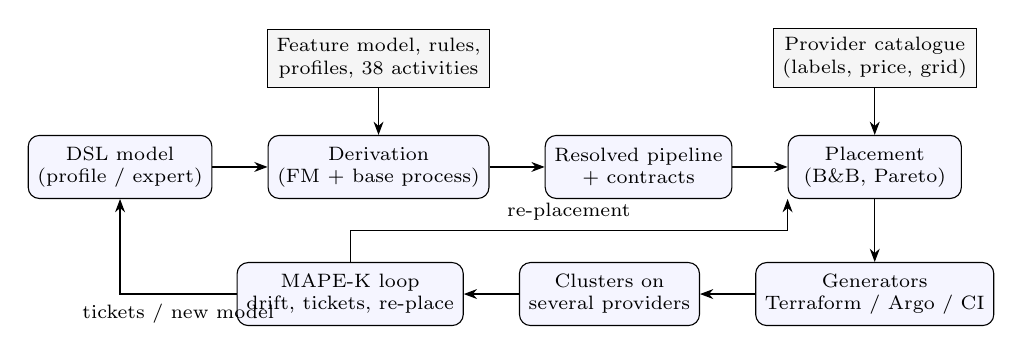
\begin{tikzpicture}[node distance=4mm and 7mm, every node/.style={font=\scriptsize,align=center},
  box/.style={draw,rounded corners,minimum width=22mm,minimum height=8mm,fill=blue!4},
  kb/.style={draw,minimum width=22mm,minimum height=7mm,fill=gray!8}, >=Stealth]
\node[box] (dsl) {DSL model\\(profile / expert)};
\node[box,right=of dsl] (der) {Derivation\\(FM + base process)};
\node[box,right=of der] (pim) {Resolved pipeline\\+ contracts};
\node[box,right=of pim] (pl) {Placement\\(B\&B, Pareto)};
\node[box,below=8mm of pl] (gen) {Generators\\Terraform / Argo / CI};
\node[box,left=of gen] (run) {Clusters on\\several providers};
\node[box,left=of run] (mape) {MAPE-K loop\\drift, tickets, re-place};
\node[kb,above=6mm of der] (fm) {Feature model, rules,\\profiles, 38 activities};
\node[kb,above=6mm of pl] (cat) {Provider catalogue\\(labels, price, grid)};
\draw[->] (dsl)--(der); \draw[->] (der)--(pim); \draw[->] (pim)--(pl); \draw[->] (pl)--(gen);
\draw[->] (gen)--(run); \draw[->] (run)--(mape); \draw[->] (mape.west) -| (dsl.south) node[pos=.25,below]{tickets / new model};
\draw[->] (mape.north) -- ++(0,4mm) -| (pl.south west) node[pos=.25,above]{re-placement};
\draw[->] (fm)--(der); \draw[->] (cat)--(pl);
\end{tikzpicture}
\caption{The \tool{} tool chain.}\label{fig:overview}
\end{figure}

\section{Knowledge layer}
\paragraph{Feature model.} The reference model has \NFeatures{} features (\NLeaves{}
leaves) and \NConstraints{} cross-tree constraints. Its six top-level subtrees are
the categories of~\cite{elhatimi2025}: \emph{Functional} (ML task, pre-processing,
tuning, explainability), \emph{Behavioral} (training triggers, deployment
strategy, human gate), \emph{Technical} (orchestrator, serving, tracking, data
versioning, runtime, GPU), \emph{Domain-specific}, \emph{Non-functional}
(objectives, monitoring signals) and \emph{Organizational} (residency,
SecNumCloud, compliance frames). The constraint reported in the consortium's poster,
\(\neg(\textit{ClassificationBaseline} \wedge \textit{DimReduction})\), is included
verbatim; others encode semantic dependencies, e.g.\ a drift trigger requires a
drift signal, a high-risk system under the AI Act requires a human gate and
explainability, HDS hosting implies a residency constraint. The leaf features are
an initial proposal by the industrial partner, to be validated by the consortium.

Configuration completion (R8) is a depth-first search over undecided features in
pre-order with Kleene three-valued evaluation of all structural rules and
constraints for pruning; it returns a minimal completion (false-first except for
features flagged as defaults) or reports the violated rules.

\paragraph{Best-practice rules.} Know-how that should not be a hard constraint is
stored as \NRules{} advisory rules, each with a condition, a rationale, a source
and, when possible, an automatic fix expressed as a feature delta. A fix is
proposed only if the resulting configuration is valid. For instance, BP01 fires
when retraining is drift-triggered without data versioning, which would make
automatic retraining non-reproducible.

\paragraph{Profiles.} \NProfiles{} profiles are named partial configurations (e.g.\
\emph{regulated-health-classifier}) that act as low-code entry points.

\section{DSL and derivation}
The concrete syntax is YAML. A minimal model and an expert refinement are shown in
Listing~\ref{lst:dsl}. The abstract syntax distinguishes the user model from the
resolved pipeline (steps typed by SkeltyMLOps activities, triggers, contracts,
objectives, placement constraints).

\begin{lstlisting}[style=yaml,caption={Non-expert model (top) and excerpt of an expert model (bottom).},label=lst:dsl]
pipeline: churn-prediction
profile: tabular-classification-continuous
data: {source: "s3://datalake/crm/churn.parquet", volume_gb: 40}
objectives: {cost: 0.6, carbon: 0.4}
---------------------------------------------------------------
profile: anomaly-detection-edge-iot
best_practices: true            # apply the advisor's automatic fixes
features: {select: [CarbonAware, GPU, HyperparameterTuning, EUResidency]}
placement: {allowed_providers: [scaleway, ovhcloud, outscale], colocate: [[serve, monitor]]}
steps:
  - {id: window_features, kind: transform, activity: D5, after: remove_outliers}
  - {id: train, hours: 3, params: {algorithm: isolation_forest}}
triggers: [{type: drift, detector: ks, threshold: 0.1}]
overrides: {steps.serve.replicas: 3}
\end{lstlisting}

Derivation (i) completes the configuration from the profile and user selections;
(ii) optionally applies valid best-practice fixes; (iii) instantiates a base
process whose variation points are bound by features: \emph{Preprocess} expands into
one step per selected pre-processing feature, \emph{Deploy} depends on the
deployment strategy (a test deployment is inserted for canary, shadow and
blue-green), \emph{Serve} is online or batch, \emph{Monitor} carries the selected
signals; optional steps (tuning, explanation, human approval) follow optional
features; (iv) merges user steps by identifier, inserting new ones in the chain;
(v) applies dotted-path overrides; (vi) derives triggers and coordination
contracts from behavioural features and placement labels from organisational
features. Every produced element records a trace link to its cause. New step kinds
and generators are registered through Python entry points, which covers
domain-specific extensions (R6) without changing the DSL.

\paragraph{Executable coordination contracts.} SkeltyMLOps describes contracts in
prose~\cite{daoud2026}. We give them an operational semantics: a ticket opened under
a contract advances gate by gate only when the gate's owner submits the required
artefacts and, if requested, an explicit approval; conditional gates (e.g.\
\texttt{model.input\_schema != api.current\_schema} for the API-impact gate) are
evaluated on the ticket context and skipped when false; every transition is
appended to an auditable trace. The derived drift-response contract reproduces the
walkthrough of~\cite{daoud2026}; the human gates are active only when the
\emph{HumanGate} feature is selected, which the AI Act constraint enforces.

\section{Placement and generation}
\paragraph{Static placement.} Each step \(s\) has resource needs and a monthly
usage; each offer \(o\) has a price, a power draw, a PUE, a grid carbon intensity,
a latency and labels. With \(x_s\) the chosen offer, we minimise
\[
J = w_c\frac{\sum_s \mathrm{cost}(s,x_s)+\sum_{(a,b)}\mathrm{egress}(a,x_a,x_b)}{C_{\mathrm{ref}}}
  + w_g\frac{\sum_s \mathrm{kWh}(s,x_s)\cdot \mathrm{grid}(x_s)}{G_{\mathrm{ref}}}
  + w_l\frac{\sum_{s\in\mathrm{serve}}\mathrm{lat}(x_s)}{L_{\mathrm{ref}}}
\]
subject to resource fit, required labels, allowed providers, pins, co-location
groups and a latency bound. The references are sums of per-step minima, so \(J\ge 1\)
when \(\sum w=1\), and \(J=1\) means every step is at its individual optimum.
We solve it exactly by depth-first branch and bound in topological order, with the
admissible bound ``partial objective + sum of per-step minima'' (egress is
non-negative) and a location-level dominance reduction (per step only the best
offer of each location can be optimal). Optimality was checked against brute force
in the test suite. A weight sweep yields the cost--carbon Pareto front.

\paragraph{Generation.} Terraform is emitted with native Scaleway resources
(Kapsule cluster, private network, node pools, versioned bucket) and module stubs
for other providers. For each location a Kubernetes cluster hosts an Argo
WorkflowTemplate with the batch steps placed there; the human gate becomes an Argo
\texttt{suspend} node; cross-location hand-offs are Argo Events webhooks and
sensors; schedule triggers become CronWorkflows and drift triggers sensors fed by
the monitor; serving and monitoring become Deployments (or a KServe
InferenceService) with ConfigMaps holding the drift policy and the contracts. A
GitHub Actions workflow re-generates the artefacts, fails on diff (the model is
the source of truth), validates Terraform and schema-checks manifests. A
\texttt{trace.json} maps each file to the model elements and activities it realises.

\paragraph{Run-time adaptation.} A MAPE-K loop monitors production batches with
PSI and two-sample Kolmogorov--Smirnov detectors, opens a ticket under the matching
contract, and compares the current placement with a re-optimised one under new
conditions. For the dynamic study we consider the serving group (serve and monitor,
co-located) and drift-triggered retraining jobs, and four policies:
\emph{static} (placed on mean conditions, moves only on outage and then returns),
\emph{reactive} (follows the hourly argmin, retrains immediately at the best
location), \emph{hysteresis} (migrates only if the forecast gain over a look-ahead
window exceeds the migration cost times \(1+m\); retraining jobs are shifted within
their deferrable window to the lowest forecast objective), and a clairvoyant
\emph{oracle} (dynamic programming over locations with switching costs, true future
values for jobs), which is a lower bound rather than a policy. Forecasts are
seasonal-naive (value 24\,h earlier).

\section{Evaluation}
\paragraph{Setup.} Four illustrative case studies: churn prediction (non-expert,
5 DSL lines), clinical triage support (regulated profile, 5 lines), predictive
maintenance on industrial IoT (expert, 28 lines) and retail demand forecasting
(expert, batch, 16 lines). The provider catalogue contains \NOffers{} offers in
\NLocations{} locations of four provider archetypes (two French clouds, a
SecNumCloud/HDS-qualified provider, a hyperscaler). \emph{All prices, power draws and
grid intensities are order-of-magnitude placeholders, not quotes}; environment traces
(hourly grid intensity with diurnal profiles, solar dips and AR(1) noise, random
outages) are synthetic and seeded. Results characterise the method, not providers.

\paragraph{RQ1 --- Knowledge coverage.} We flip each leaf feature in the context of
a reference profile and check whether the derived model or the generated artefacts
change (Table~\ref{tab:features}). \FeatTested{} of \FeatLeaves{} leaves can be
flipped consistently; \FeatEffective{} have an observable effect. Behavioural,
non-functional and organisational features are all effective. The inert ones are
\FeatNoEffect{}: they reveal that the current generators target only Argo on
Kubernetes and emit nothing for data versioning or experiment tracking, and that
the ML task and some domains do not yet change the pipeline. This metric turns the
feature model into a test oracle for generator completeness.

\begin{table}[t]\centering\small
\caption{Leaf features per category: total, consistently flippable, and with an observable effect on the output.}\label{tab:features}
\begin{tabular}{lrrr}\toprule
Category & Leaves & Tested & Effective\\\midrule
\csname @@input\endcsname generated/tab_features.tex 
\bottomrule\end{tabular}
\end{table}

Regarding the reference architecture, generated artefacts realise \CovTotal{}
SkeltyMLOps activities: Ops \CovOps, Data \CovData, Model \CovModel, Soft \CovSoft,
Plan \CovPlan. Plan activities (conceptualising, requirements, architecture
design) are human by nature and are supported by the DSL itself rather than by
generated code; the uncovered Data, Model and Soft activities (collecting and
labelling data, experimenting, developing model code, building and packaging) are
the developer-side work that a deployment DSL deliberately leaves to users.

\paragraph{RQ2 --- Pivotal model.} Table~\ref{tab:abstraction} relates model size to
generated artefacts. A 5-line non-expert model yields 10--11 steps and about 400
lines of Terraform, Argo and CI configuration; expert models are larger (they
carry parameters) and the ratio drops to \RatioMin. Line ratios are only a proxy for
effort; they do not measure correctness of the generated code, which we check by
parsing all manifests, asserting DNS-compatible Argo names and native Terraform
resources in the test suite, but not yet by deployment on real clusters.

\begin{table}[t]\centering\small
\caption{Model size vs.\ generated artefacts (non-comment lines). Findings: fired best-practice rules.}\label{tab:abstraction}
\begin{tabular}{lrrrrrr}\toprule
Case & DSL lines & Steps & Files & Generated lines & Ratio & Findings\\\midrule
\csname @@input\endcsname generated/tab_abstraction.tex 
\bottomrule\end{tabular}
\end{table}

\paragraph{RQ3a --- Static placement.} Table~\ref{tab:placement} compares the
optimum with single-provider optima and with a cost-only placement. Three
observations. (1) The multi-provider optimum equals the best single-provider
optimum (to three decimals) in all cases: the value lies in choosing the right
provider and region per pipeline, not in splitting a pipeline, because egress and
co-location penalise splits. (2) Choosing badly is expensive: the worst feasible
single provider has an objective up to 35\% above the optimum (churn: 1.470 vs.\ 1.086). (3) Carbon-aware
weights cut operational carbon by \CarbonSavingChurn\% (churn) and
\CarbonSavingRetail\% (retail) versus the cost-only placement for
+\CostExtraChurn\% and +\CostExtraRetail\% cost; this gap is driven by the
catalogue's cheaper, high-carbon region and must be re-measured with real prices.
For the regulated case, the HDS label leaves a single feasible provider.
The exact solver needs 91--271 nodes on chains of 10--30 steps; ties between
near-equivalent French regions raise this to \(3.4\times10^5\) nodes (a few seconds)
for the maintenance case.

\begin{table}[t]\centering\scriptsize
\caption{Static placement. Cost in EUR/month, carbon in kgCO\(_2\)e/month, \(J\) normalised objective (1 = per-step optimum).}\label{tab:placement}
\begin{tabular}{lrrrrrrrrr}\toprule
Case & Providers & Cost & Carbon & \(J\) & \(J\) best single & \(J\) worst single & Cost (cost-only) & Carbon (cost-only) & B\&B nodes\\\midrule
\csname @@input\endcsname generated/tab_placement.tex 
\bottomrule\end{tabular}
\end{table}

\begin{figure}[t]\centering
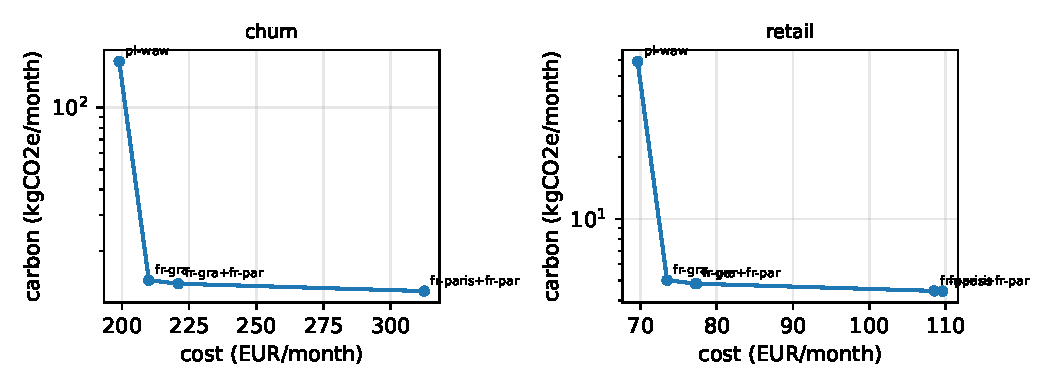
\includegraphics[width=.9\linewidth]{figures/pareto.pdf}
\caption{Cost--carbon Pareto fronts (weight sweep); labels are the regions used.}\label{fig:pareto}
\end{figure}

\paragraph{RQ3b --- Dynamic re-deployment.} We simulate 30 days (hourly) for the
maintenance pipeline with equal cost and carbon weights, 20 seeds, in two scenarios:
A, all EU locations allowed; B, French locations excluded (e.g.\ a residency
constraint towards other EU countries), leaving two serving locations whose grids
differ in daily shape. Table~\ref{tab:dynamic} reports means over seeds; \(J\) is
normalised by the static policy of the same seed.

\begin{table}[t]\centering\small
\caption{Dynamic policies over 30 days (mean \(\pm\) sd over 20 seeds). Job carbon: drift-triggered retraining only.}\label{tab:dynamic}
\begin{tabular}{llrrrrr}\toprule
Scen. & Policy & Cost (EUR) & Carbon (kg) & Migrations & \(J\) & Job carbon (kg)\\\midrule
\csname @@input\endcsname generated/tab_dynamic.tex 
\bottomrule\end{tabular}
\end{table}

The upside of hourly re-placement is small: the clairvoyant oracle improves \(J\)
by only 1.7\% (A, \(J=\JAOracle\)) and 0.7\% (B, \(J=\JBOracle\)) with 2--3 migrations a month. The
reactive policy migrates \MigAReactive{} (A) and \MigBReactive{} (B) times a month;
it saves \CarbonAReactivePct\% and \CarbonBReactivePct\% of carbon but raises cost by
\CostAReactivePct\% and \CostBReactivePct\%, hence \(J=\JAReactive\) and \JBReactive.
Hysteresis avoids this churn (\(<1\) migration a month) but does not capture the
oracle's gain: \(J=\JAHyst\) and \JBHyst. The ablation (Table~\ref{tab:ablation})
shows the same picture for margins 0--1 and look-aheads of 3--12\,h. A diagnosed
weakness is that, after a forced move caused by an outage, hysteresis only returns if
the short-horizon forecast gain covers the migration cost, which the static policy
does unconditionally; this explains its higher carbon variance in scenario B.
Temporal shifting of retraining jobs is where flexibility pays in relative terms:
job carbon drops by \JobCarbonAPct\% (A) with a 12\,h window, and the oracle shows
that better forecasts could reach about 20\%; retraining is however a small share of
the total here.

\begin{table}[t]\centering\small
\caption{Hysteresis ablation, scenario B (10 seeds).}\label{tab:ablation}
\begin{tabular}{rrrr}\toprule Margin \(m\) & Look-ahead (h) & \(J\) & Migrations\\\midrule
\csname @@input\endcsname generated/tab_ablation.tex 
\bottomrule\end{tabular}
\end{table}

\begin{figure}[t]\centering
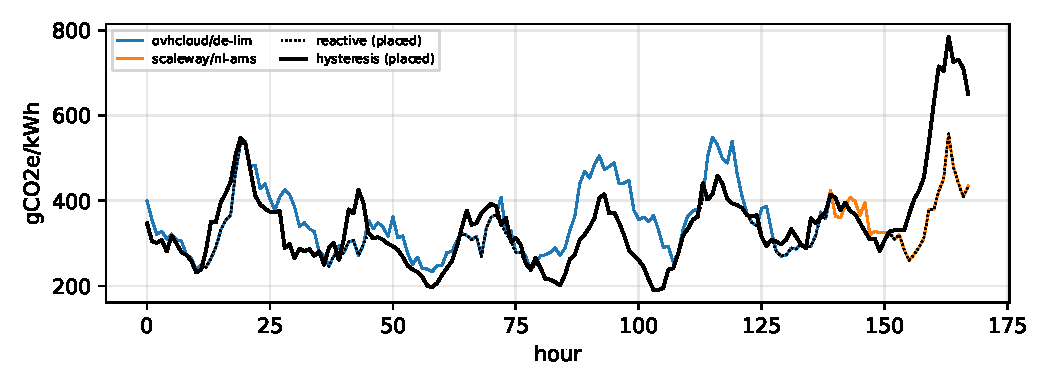
\includegraphics[width=.9\linewidth]{figures/trace_B.pdf}
\caption{Scenario B, first week, seed 0: grid intensity of the two feasible serving locations and intensity experienced by the placed service.}\label{fig:trace}
\end{figure}

\section{Discussion}
\paragraph{For tool design.} Under these assumptions, the placement decision that
matters is the initial, constraint- and objective-aware choice of provider and
region; it should be made explicit and traceable at design time, which the DSL does.
Dynamic re-placement of long-running services should be conservative by default,
triggered by events (outages, price or catalogue changes, drift-induced retraining)
rather than by hourly signals; temporal shifting of deferrable training is the
cheap lever. These are statements about the method on synthetic inputs; the
magnitudes will change with real traces, larger state to migrate, or regions with
more volatile grids.

\paragraph{Relation to the consortium's work.} The prototype reuses the six
variability categories, the requirements R1--R8 and the SkeltyMLOps activities and
contracts. It addresses R2, R5, R7, R8 through the feature model and derivation,
R1 and R4 through triggers, conditional gates and Argo DAGs, R3 and R6 through
step-kind and generator registries. It does not yet offer a BPMN or graphical
process view, nor a metamodel in a standard MDE technical space (e.g.\ Ecore); both
are natural bridges to the academic partners' work.

\section{Threats to validity}
\emph{Construct}: \(J\) aggregates heterogeneous criteria through weights and
per-step references; lines of generated code are a weak proxy for effort; carbon is
operational and location-based only (no embodied emissions, no network energy).
\emph{Internal}: the leaf features, rules and constraints are the author's proposal
and have not yet been validated by the consortium; migration cost is a fixed
penalty plus egress. \emph{External}: prices, power draws and grid intensities are
placeholders and the environment is synthetic; case studies are illustrative, not the
industrial cases announced in the project. \emph{Conclusion}: 20 seeds give tight
intervals on synthetic data but say nothing about real variability. Generated
artefacts are parsed and unit-tested, not yet deployed.

\section{Conclusion and roadmap}
We presented \tool, a variability-aware low-code DSL that compiles MLOps pipelines
to multi-provider IaC/PaC and adapts them at run time, grounded in the variability
and reference-architecture results of the AdaptiveMLOps consortium. Next steps are:
(1) consortium review of the feature model and rules; (2) replacement of the
catalogue and traces by contractual prices and measured grid data, and deployment
of generated artefacts on the industrial partner's platform; (3) generators for
experiment tracking, data versioning and alternative orchestrators, guided by the
inert-feature metric; (4) a return-to-preferred-location rule and event-driven
triggers for re-placement; (5) an Ecore metamodel and a BPMN view aligned with the
process-line modelling of the academic partners; (6) evaluation with non-expert
users.

\section*{Data and code availability}\label{sec:availability}
Source code, examples, tests and the experiment script (\texttt{experiments/run\_all.py})
are provided in the accompanying repository under Apache-2.0. All tables, figures and
numbers in this paper are produced by that script (\texttt{paper/generated/}).

\section*{Acknowledgements}
This work is part of the AdaptiveMLOps project funded by the French National Research
Agency (ANR-24-IAS2-0004).

\section*{Declaration on generative AI}
A large language model assistant was used to help write code and draft this text;
the author reviewed the design, the code, the experiments and the manuscript and takes
responsibility for the content.

\begin{thebibliography}{99}\small
\bibitem{kreuzberger2023} D.~Kreuzberger, N.~Kühl, S.~Hirschl. Machine Learning Operations (MLOps): Overview, definition, and architecture. \emph{IEEE Access} 11:31866--31879, 2023.
\bibitem{sculley2015} D.~Sculley et al. Hidden technical debt in machine learning systems. \emph{NeurIPS}, 2015.
\bibitem{gama2014} J.~Gama, I.~Žliobaitė, A.~Bifet, M.~Pechenizkiy, A.~Bouchachia. A survey on concept drift adaptation. \emph{ACM Computing Surveys} 46(4), 2014.
\bibitem{elhatimi2025} C.~El Hatimi, V.~Berry, A.-D.~Seriai, V.~Preney, X.~Quesnot, C.~Tibermacine, C.~Urtado, S.~Vauttier. Toward Adaptive MLOps: Variability mapping and modeling. \emph{Journées nationales du GdR GPL}, Pau, 2025. hal-05127859.
\bibitem{daoud2025} C.~Daoud, D.~Azar, J.~Boiché, C.~Urtado, S.~Vauttier. SkeltyMLOps: Orchestrating collaborative MLOps activities. \emph{MLOps25 Workshop, ECAI 2025}, pp.~55--66. hal-05337700.
\bibitem{daoud2026} C.~Daoud, D.~Azar, C.~Urtado, S.~Vauttier. A reference architecture for an orchestrated collaborative MLOps: A ground-up design from literature combining human and LLM expertise. \emph{Future Generation Computer Systems} 185:108700, 2026.
\bibitem{kang1990} K.~C.~Kang, S.~G.~Cohen, J.~A.~Hess, W.~E.~Novak, A.~S.~Peterson. Feature-Oriented Domain Analysis (FODA) feasibility study. CMU/SEI-90-TR-21, 1990.
\bibitem{batory2005} D.~Batory. Feature models, grammars, and propositional formulas. \emph{SPLC}, 2005.
\bibitem{benavides2010} D.~Benavides, S.~Segura, A.~Ruiz-Cortés. Automated analysis of feature models 20 years later: A literature review. \emph{Information Systems} 35(6), 2010.
\bibitem{osterweil1987} L.~Osterweil. Software processes are software too. \emph{ICSE}, 1987.
\bibitem{terenciani2015} M.~Terenciani, D.~M.~B.~Paiva, G.~B.~Landre, M.~I.~Cagnin. BPMN* -- A notation for representation of variability in business process towards supporting business process line modeling. \emph{SEKE}, 2015.
\bibitem{najafabadi2024} F.~Amou Najafabadi, J.~Bogner, I.~Gerostathopoulos, P.~Lago. An analysis of MLOps architectures: A systematic mapping study. \emph{ECSA}, 2024.
\bibitem{colantoni2020} A.~Colantoni, L.~Berardinelli, M.~Wimmer. DevOpsML: Towards modeling DevOps processes and platforms. \emph{MODELS Companion}, 2020.
\bibitem{rahman2019} A.~Rahman, R.~Mahdavi-Hezaveh, L.~Williams. A systematic mapping study of infrastructure as code research. \emph{Information and Software Technology} 108, 2019.
\bibitem{wiesner2021} P.~Wiesner, I.~Behnke, D.~Scheinert, K.~Gontarska, L.~Thamsen. Let's wait awhile: How temporal workload shifting can reduce carbon emissions in the cloud. \emph{Middleware}, 2021.
\bibitem{radovanovic2023} A.~Radovanović et al. Carbon-aware computing for datacenters. \emph{IEEE Transactions on Power Systems} 38(2), 2023.
\bibitem{kephart2003} J.~O.~Kephart, D.~M.~Chess. The vision of autonomic computing. \emph{Computer} 36(1), 2003.
\end{thebibliography}
\end{document}
